\documentclass[a4paper,12pt]{article} % This defines the style of your paper

\usepackage[top = 2.5cm, bottom = 2.5cm, left = 2.5cm, right = 2.5cm]{geometry} 

\usepackage[T2A]{fontenc}
\usepackage[utf8]{inputenc}
\usepackage[russian]{babel}

\usepackage{multirow} 
\usepackage{booktabs} 

\usepackage{graphicx} 

\usepackage{setspace}
\setlength{\parindent}{0in}

\usepackage{float}

\usepackage{amsmath}

\usepackage{fancyhdr}

\usepackage{pgfplots}
\pgfplotsset{compat=1.9}

\pagestyle{fancy} 

\fancyhf{} 

\lhead{\footnotesize Расчетное задание №16}

\rhead{\footnotesize Николаев Юрий} 

\cfoot{\footnotesize \thepage} 

\begin{document}

\thispagestyle{empty} 

\begin{tabular}{p{15.5cm}} 
НИУ МЭИ \\ А-13а-19  \\ Вариант 13 \\ Николаев Юрий\\
\hline 
\\
\end{tabular} 

\vspace*{0.3cm}

\begin{center} 
	{\Large \bf Расчетное задание №16} 
	\vspace{2mm}
\end{center}  

\vspace{0.4cm}


\section{Задание}
Функция $y = y(x)$ задана таблицей своих значений.Вычислить приближенное значение функции в точке $\bar x$, используя интерполяционные многочлены Ньютона первой, второй и третьей степеней. Для каждого вычисленного значения найти практическую оценку погрешности. Записать все результаты с учетом погрешности.

\vspace{0.4cm}

УКАЗАНИЕ. Перед построением многочленов следует переупорядочить таблицу, расположив точки в порядке удаления от $\bar x$.

$$\bar x = 5,38$$

\begin{center}
\begin{tabular}{| c | c | c | c | c | c |}
\hline
    x & 4 & 4,4 & 5,2 & 5,6 & 6,4 \\ \hline
    y & 19 & 22,5 & 30,3 & 34,7 & 44,5 \\
\hline
\end{tabular}
\end{center}

\section{Решение}

\begin{enumerate}

\item Построим многочлен Ньютона $P_n(x)$:

Упорядочим узлы в порядке возрастания расстояния от точки $\bar x$:
\begin{center}
\begin{tabular}{ c  c  c  c  c }

    $x_0 = 5,2;$ & $x_1 = 5,6$ & $x_2 = 4,4$ & $x_3 = 6,4$ & $x_4 = 4$ 

\end{tabular}
\end{center}

Составим диагональную таблицу разделенных разностей:

\begin{center}
\begin{tabular}{| c | c | c | c | c | c |}
\hline
    $x_i$ & $y_i$ & $y(x_0, x_1)$ & $y(x_0, x_1, x_2)$ & $y(x_0, x_1, x_2, x_3)$ & $y(x_0, x_1, x_2, x_3, x_4)$ \\ \hline
    5,2 & 30,3 &  &  &  &  \\ \hline
      &  & 11 &  &  &  \\ \hline
    5,6 & 34,7 &  & 1,04125 &  &  \\ \hline
      &  & 10,167 &  & 0 &  \\ \hline
    4,4 & 22,5 &  & 1,04125 &  & -0,05404 \\ \hline
      &  & 11 &  & 0,06484 &  \\ \hline
    6,4 & 44,5 &  & 0,9375 &  &  \\ \hline
     &  & 10,625 &  &  &  \\ \hline
    4 & 19 &  &  &  &  \\
\hline
\end{tabular}    
\end{center}

Многочлен Ньютона первой степени:
$$
P_1(x) = 30,3 + 11(x - 5,2)
$$

$$
P_1(5,38) = 32,28
$$

Многочлен Ньютона второй степени:
$$
P_2(x) = 30,3 + 11(x - 5,2) + 1,04125(x - 5,2)(x - 5,6)
$$

$$
P_2(5,38) = 32,2388
$$

Многочлен Ньютона третьей степени:
$$
P_3(x) = 30,3 + 11(x - 5,2) + 1,04125(x - 5,2)(x - 5,6) + 0(x - 5,2)(x - 5,6)(x - 4,4)
$$

$$
P_3(5,38) = 32,2388
$$

Многочлен Ньютона четвертой степени (нахожу для оценки погрешности):
$$
P_4(x) = 30,3 + 11(x - 5,2) + 1,04125(x - 5,2)(x - 5,6) - 0,05404(x - 5,2)(x - 5,6)(x - 6,4)(x - 4,4)
$$

$$
P_4(5,38) = 32,236627
$$

Найдем погрешность: 
$$R_1(5,38) = 32,28 - 32,2388 = 0,0412$$
$$R_3(5,38) = 32,2388 - 32,236627 = 0,002173$$

Получим ответы: 
$$f(5,38) = 32,280 \pm 0,041$$
$$f(5,38) = 32,239 \pm 0,002$$

\newpage

\begin{figure}[h]
\center{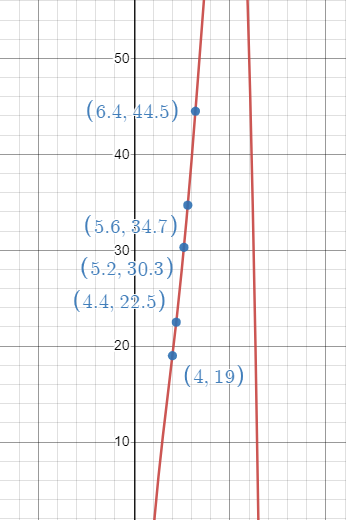
\includegraphics[scale=1]{graphic16.png}}
\caption{График многочлена и исходных точек}
\label{fig:image}
\end{figure}

\end{enumerate}

\end{document}